\documentclass[letterpaper]{article} % Feel free to change this
\usepackage{graphicx}
\usepackage{float}
\begin{document}

\title{ECE 350: Digital Systems Project Checkpoint 4}
\author{Jack Fitzpatrick} % Change this to your name
\date{3/4/17} % Change this to the date you are submitting
\maketitle

\section*{Duke Community Standard}

By submitting this \LaTeX{} document, I affirm that
\begin{enumerate}
    \item I understand that each \texttt{git} commit I create in this repository is a submission
    \item I affirm that each submission complies with the Duke Community Standard and the guidelines set forth for this assignment
    \item I further acknowledge that any content not included in this commit under the version control system cannot be considered as a part of my submission.
    \item Finally, I understand that a submission is considered submitted when it has been pushed to the server.
\end{enumerate}

\section*{Introduction}
This technical document describes the included Verilog processor, how it was designed, which instructions were implemented, and the overall process of creating it. The processor is a five stage, 32-bit pipelined processor with hardware interlocks, which implements the "ECE 350 ISA," shown in Appendix A. Currently, the processor implements every instruction specified, with a couple bugs related to bypassing and stalling for multiplication, division, branching, and loading words. There are a few register conventions consistent with this processor. Register \$r31 is written to during a jump and link (jal) operation. Register \$r30 is the status register, which is written to and read from when error statuses are concerned. Finally, Register \$r0 will always contain the value 0.
\newpage
\section*{Submodules and Project Checkpoints}
This section outlines the main submodules present in this processor. The three main submodules, the Regfile, ALU, and MultDiv, were previously submitted for previous Project Checkpoints. The original versions did contain some bugs, which have since been eliminated. \\

\subsection*{Regfile}
The regfile contains 32 32-bit registers. One register can be written to, and two can be read from in one clock cycle. The registers themselves are composed of 32 d flip flops, which have enable and asynchronous reset inputs, written with behavioral verilog. The input write register control signal is passed through a decoder, which converts the 5-bit encoded input into a 32-bit decoded output, with only 1 corresponding bit asserted. This decoded sequence is passed to each respective register as its input enable, so that only the specified register will write the input data to its d flip flops (with the exception of \$r0). The decoder is made from 32 and gates, which hard-code the decoder logic. To output data from the desired register, each register's 32-bit output bus is passed through 2 multiplexers, with the read register A and B control signal as the multiplexer's chooser. The correct bus will then be output from the multiplexer. The multiplexers are made hierarchically, starting from a 2-input mux, created from two sets of 32 and gates which "choose" the desired input. Each subsequent multiplexer is built from two previous multiplexers, and one 2-input mux. The highest-level mux has 32 inputs, for the 32 registers. \\

\subsection*{ALU}
The ALU has 6 required functions: addition, subtraction, bitwise and, bitwise or, shift left logical, and shift right arithmetic, determined by an ALU opcode. Additionally, when subtracting, the ALU had to determine if A did not equal B, and if A was less than B, where A and B are the ALU's two inputs. These functions were implemented with 5 general submodules: a carry lookahead adder, 32 and gates, 32 or gates, and two barrel shifters. The output of the ALU is determined using a multiplexer, copied from the Regfile, which uses the opcode as the control signal, and outputs the correct submodule's output.  \\
\begin{enumerate}
\item The carry lookahead adder block was built with four 8-bit lookahead blocks, implementing carry lookahead logic. This logic determined if each individual bit within a block would either propagate or generate a carry bit. The blocks themselves would also have propagate or generate values, which are used to predict the carries between blocks. This produces an adder with a reduced cost function from a typical ripple carry adder. The adder block can also handle subtraction. For subtraction, the adder simply inverts the 2's compliment B input, by inverting each individual bit, and asserting the carry-in bit to the adder. This simulates subtraction for 2's compliment numbers. \\
\item The bitwise AND and OR blocks are fairly straightforward. The inputs are simply passed through 32 AND or OR gates. \\
\item The barrel shifters are two separate modules, but are constructed in a very similar way. The only difference is the direction of the shift and whether or not the bit is extended (it is in arithmetic shifts, not logical shifts). For each shifter, there are 5 submodules which shift their inputs by 1, 2, 4, 8, and 16 bits. Each submodule has an enablt bit, which determines whether or not it will shift the input. The shifters are enabled based on the shift amount input. If shiftAmt[0] is asserted, then the 1 bit shifter's enable bit is asserted. If shiftAmt[1] is asserted, then the 2 bit shifter's enable bit is asserted, and so on. This will shift the input by the requested amount, once every shifter acts upon it. \\
\item The "is not equal" and "is less than" bits are valid only if subtraction has been performed. If it has, is not equal simply checks the output. If the output is 0, then the two inputs are equal, so "is not equal" is 0. Otherwise it is 1. Similarly, if the result is negative, A must have been less than B, so "is less than" is asserted. Otherwise it is not. \\
\item The overflow output is true for three conditions, which are checked within the adder module: two negative numbers are added to make a positive one, two positive values are added to make a negative one, and a negative A operand subtracted by a positive B operand produces a positive number. Otherwise, overflow is 0. \\
\end{enumerate}
The ALU submitted for the Project Checkpoint had issues with the "did not equals" output. The problem was a syntax error, where instead of checking if the entire output was 0, only the first bit was checked. Fortunately, this caused the ALU to pass half the tests, so not all was lost. \\
\newpage
\subsection*{MultDiv}
My implementation of MultDiv was a finite state machine that utilized Booth's algorithm for multiplication and a naive method for division. They use the same registers for storing their states, as well as the same counter. A ready output is asserted when the counter is done, and the result is ready. It takes 32 cycles to complete. \\
\begin{enumerate}
\item The counter register is a 6-bit register which counts to 32. Every clock cycle, it uses a simple adder to add 1 to its value. At 32, it no longer counts, and asserts a ready signal if no exceptions occurred. It is reset if either the mult or div control input is asserted, signifying an interrupt to the previous operation. \\
\item The product/RQB register is a 64 bit register made from d flip flops, similar to those in regfile. The register is enabled when the mult or div control inputs are asserted, or when the counter is actively counting. Booth's algorithm is implemented with an additional d flip flop, acting as a buffer to store the extra bit. The buffer and last bit of the product register is examined each cycle, and the multiplicand is added or subtracted to the top 32 bits of this register if necessary, using a carry lookahead adder copied from ALU. For division, the adder is used to compare the remainder and divisor, and if the remainder is larger, the divisor is subtracted from the remainder and the quotient is updated. It is a naive divider, so both inputs are made positive to begin, and the result is made negative if necessary. \\
\ item There is a 1 bit state register used to keep track of which operation is occurring. 0 is multiplication, 1 is division. \\
\item Shifters used to shift the product/RQB register are simply implemented with $<<<$ and $>>>$ operators. \\
\item There are two inverters included, which invert the inputs for division if necessary. These modules simply invert each bit and add one to the result.
\item Exceptions occur when two max-value numbers (\(2^{32}-1\)) are multiplied together, or a number is divided by 0. These conditions are determined with 0 and max checkers, implemented with simple AND and NOT logic gates. \\
\end{enumerate}
My MultDiv was mostly functional for the Project Checkpoint. However, since it was not negatively clocked, causing hold time violations. That has since been fixed.


\subsection*{Memory Elements}
The instruction memory (read-only) and data memory (read and write) were generated with Altera's syncram megafunction, which can generate 32-bit, word addressed, 1-port, 50 MHz ROM or RAM. The implementation of these memory elements was specified in the provided skeleton code. They are initialized from mif or hex files with their initial memory values. The instruction memory begins executing at instruction 0, although this should be a no op due to edge cases with resets. The regfile, data memory, and instruction memory are all negatively clocked, while the latches within the processor itself are positively clocked. This was done to offset memory access and processor execution, so that processor signals to memory were stable when that memory is written, and vice versa.

\subsection*{Other Processor Submodules}
There are various other submodules in use in this processor. The branch adder is a simple 12-bit adder used in the Execute stage to calculate the new PC value on a branch. The address comparer takes two register values, and returns 1 if they are equal, for use with data hazard checking. It returns 0 if either is 0, as data hazards are not concerned with the 0 register. Finally, the get status module takes the instruction value and exception bit as input, and returns the proper error status. This could be 0 if there is no error, 1-5 for ALU or MultDiv errors, and custom if setx is called. \\

\section*{Full Processor Implementation}
The full processor is a five stage, hardware interlocked processor. The five stages include Fetch, Decode, Execute, Memory, and Writeback (F, D, X, M, and W), and the transitions between them. The transitions are positively clocked registers which hold the necessary values, such as instruction and ALU output data. The processor can be clocked at 50 MHz without timing issues.\\

\subsection*{Fetch}
This stage is responsible for fetching the correct instruction to execute. It contains a 12 bit PC register, which is used to store the address of the current instruction in instruction memory. The input of this register is determined from a mux, and it can either be itself incremented by 1 word (which is the default), or a specific target value, if a jump or branch instruction has been called. Fetch simply reads instruction memory, gets the output, and passes it through a register to the next stage. The value of the PC is also saved for future instructions. \\

\subsection*{Decode}
In the decoding stage, values are read from the regfile, and potential hazards are caught. Hazards will be discussed later. The two registers to be read are determined based on the type of instruction being executed, deduced from the instruction value passed from the Fetch stage. The type of instruction determines if A or B should be rs, rd, or rt. I was not able to implement early branching within the Decode stage, although I attempted to. This would have reduced branch delays by one cycle, but it got too complicated, and I needed a basic implementation before I went for something more ambitious. Decode passes on the instruction value, PC value, and the two read register values. Decode also determines the immediate value for I type instructions, to alleviate pressure on the execute stage and increase efficiency. This value is also saved in a register and passed on. \\

\subsection*{Execute}
The execute stage is where the bulk of the processor lies. This stage contains the ALU, MultDiv, and most of the hazard logic. First, the ALU and MultDiv inputs are pulled from the instruction. The ALU will use its opcode for R type instructions, subtraction for branch instructions, and addition otherwise. Mult and div control inputs are set by specific opcodes for R type commands. Additionally, MultDiv has a d flip flop that tracks its progress. If the MultDiv is executing a command, it sets this register to 1, and stalls the processor until it completes. There is currently a bug that causes it to take extra time to complete, even after the value is read. The execute stage also handles branching logic. For branches and jumps, it will set the PC to a new value if the conditions are met. The PC assumes a branch is not taken, so if a branch is taken, all registers between the Fetch and Execute stages are reset to 0, using a flush signal. The Execute stage passes along the instruction, PC, ALU/MultDiv out, register B value, exception information, and hazard information to the Memory stage. \\

\subsection*{Memory}
The Memory stage accesses the data memory. The address to this memory is set to the X/M register's ALU output for store operations, or directly to the next instruction's ALU output for a load instruction, as this memory operates in a delayed way. This will cause hazards with stores immediately followed by loads, so stalls are necessary to prevent simultaneous memory access. Write enable is set to the store flag, and the data is set to the B register value. This stage passes along the instruction, PC, read memory data, ALU/MultDiv output data, and hazard/exception data. \\

\subsection*{Writeback}
Writeback first uses a submodule to get an error status. This error status, which is usually 0, is set to a certain value based on the type of instruction and exception flag, with actual exceptions taking precedent over setx commands. This is done with a series of multiplexers checking opcodes. Then, the control write register and data write register values are set according to the instruction, with the write enable value only being asserted if needed. \\

\subsection*{Stalls and Bypasses}
Hazards occur when a register is written to after being read from by a later instruction. This is detected by comparing the rd register from previous commands to other registers in current commands, depending on the type of instruction. This is done in the Decode and Execute stages. In the Decode stage, hazards for ALU inputs after loads are detected. These can't be bypassed, as the first instruction has not yet gotten to the Memory stage so the processor instead stalls for one cycle. In the Execute stage, registers are again compared to the rd registers of Memory and Writeback instructions. If any hazards are detected, the updated value of the register is acquired, with preference for the Memory stage, as it is more recent. This is done by rerouting the write register data value or the Memory ALU out data through a multiplexer, to the inputs of the ALU or MultDiv. This vastly increases efficiency, as the processor does not need to be stalled for every data hazard. There is one bypass bug, where branch commands right after load commands cause issues.  \\
Control hazards are briefly mentioned above. When a branch is taken, previous registers are flushed, so that any commands that shouldn't execute are erased. \\
In some cases, I sacrifice efficiency for accuracy. With MultDiv, jumping, branching, and sequential stores/loads, I prefer to take a hit to efficiency and stall, rather than run the risk of having errors. Given more time, I would be able to iron these issues out of the processor, but the current version is not optimized for speed. \\


\section*{Instruction Implementation}
Here are details about how each instruction was implemented.
\subsection*{R Type}
Basic R Type commands were very simple to implement. In the Decode stage, register A is set to rs, and B is set to rt. In the Execute stage, if the instructions were not mult or div, the ALU opcode, shift amount, and inputs were passed into the ALU, and the output was written to rd in the Writeback stage. For mult and div, the stall register mentioned above was set, and either the mult or div control signal was asserted. When the result is ready, it is also written into rd.

\subsection*{I Type}
There are three general I Type commands: add immediate, store/load, and branch commands.
\begin{enumerate}
\item Add immediate was implemented in the same way as add, but the second ALU input was replaced with the immediate value. The result was written to rd, as with the R type commands.
\item Store and load commands were not too difficult to implement. Like R Type and addi commands, they require rs to be register A. Store commands require rd be register B, however. Like with addi, rs is added with the immediate value, and the result is passed to the dmem address input. For store commands, register B's value was set as the data input, and write enable for dmem was asserted. For load commands, the output of dmem was saved, and written into rd.
\item Branch commands were the hardest to implement. First, register A must be set to rd, and B to rs. Then, the ALU opcode must be set to subtraction. This way, there would be valid outputs for "not equal" and "is less than." Using these results, and a branch adder module to add the lower 12 bits of the immediate value to the PC, a new "branchedPC" value was found. If the conditions of bne or blt were met, "branch" is asserted, flushing the previous registers and setting the PC to the new branched value. 
\end{enumerate}

\subsection*{JI Type}
There are two general types of JI commands: jump commands, and exception commands.
\begin{enumerate}
\item Jump commands were very easy to implement once the branch commands were established. The new branched PC value was simply set to the target value, and branch was asserted. In the case of jal, a specific register (\$r31) is set to the previous PC, which is saved throughout the pipeline. Fortunately, no data hazards can come of this, since all previous commands are flushed when a jump command is called.
\item Exception commands are fairly unique, in the sense that they only concern one register. The bex command uses a submodule that checks if \$r30 is 0. If it isn't, bex acts as a simple jump command, changing the new value of PC and asserting branch and flush. Setx is even simpler, and just sets \$30 in the Writeback stage.
\end{enumerate}

\subsection*{jr Command}
The jr command, the only JII Type command, sets the PC to a specific value, stored in the register rd. In Decode, register A is set to rd. In execute, a multiplexer is used to find the target between other J and JI type commands. If the command is jr, the value of the target is set to register A's value. The PC is then set to the value of this target, branch is asserted, and the previous registers are flushed.

\section*{Development Process}

This implementation was chosen based on the five-stage pipelined processor described in class. The basic bypass logic was taken from lecture, and slightly modified to fit. Unfortunately, Decode-stage branch calculations and branch predictions could not be implemented due to time constraints. Overall, I believe I hit a good balance between efficiency and accuracy, given the time we had for this project. \\ \\
I tested my implementation primarily with waveforms. I added three outputs to both the processor and skeleton, called probe0, probe1, and probe2, all 32 bits. I could then assign these probes to whatever value I wanted to measure and see them on the waveform. Additionally, with multiple probes, I could see simultaneous measurements from the same instruction. A common setup was to have probe1 be equal to data\_writeReg, probe2 measure ctrl\_writeReg, and probe3 measure w\_insn. This was my primary form of debugging. Additionally, finding out how to use hex within mif files helped me immensely. \\ \\
As mentioned above, I currently have small bugs in the division of MultDiv, multiple mult or div operations, and branch commands right after a load command. I found these issues by testing my processor with a stream of various commands. The delays after MultDiv operations, and between multiple ones, is due to the logic of the multiplication register that stalls the processor. It is sometimes triggered accidentally after a mult or div operation, so 32 cycles are lost. This can be fixed by redoing the register's logic. \\
Branch commands after load operations do not get updated values. This is a bypassing issue, so my bypassing logic must be reexamined. The logic around branch operations is already incredibly complex, with many interdependencies on other stages and outputs, so squashing this bug will take a lot of debugging and logic mapping. \\ 
Finally, there seems to be a bug where any command after a lw command is not registered. This is my longest lasting bug, and I have not been able to make any progress with it. At first, it seemed to be a bypassing issue, but after tracing the signal's trail, that is not the case. I believe it might have to do with the PC being faulty. \\ \\
The main challenge I faced was debugging my processor. The debugging process itself was not difficult, but the Quartus software makes it tedious. For one, since my laptop's display is 4k, it makes all the icons and scaling of the program very small, and very hard to read. Secondly, it takes my laptop quite a long time to compile my processor, and even longer to run a simulation. I end up staring at my screen for at least a minute, doing nothing, while the simulation loads. \\
Other than logistical problems, the processor posed many challenging logical problems. The many interactions between each stage and the memory elements make this assignment very complex, and the simultaneous nature of the processor executing multiple instructions is hard to wrap your head around. I overcame these issues by drawing a lot of diagrams, mapping the logic of my processor from stage to stage. There are many scribbled charts in my notebook, dissecting each instruction, finding what components of the processor it needs, and where to map rd, rs, and rt. \\ \\
Overall, this Processor assignment helped me learn how pipelined processors worked on a much deeper level. It is one thing to see the overall design, but to actually put it all together yourself helps you understand the interactions and dependencies so much more. In addition to this general knowledge, I also learned why memory elements should be negatively clocked, how multiplication works, how hazards are handled, and how processors can be made much more efficient with more hardware. \\

\section*{Conclusion}

This assignment led me to create a functioning, pipelined, 5-stage, 32-bit processor using Verilog, a hardware description language. This assignment deepened my understanding of processors, and allowed me to explore how exactly they function. Additionally, this assignment represents the culmination of my digital systems education so far: learning MIPS in 250, which led to a Logisim processor, to Verilog, and finally to this full processor, made "from scratch." The MIPS code I wrote in 250 could feasibly be run on this processor, which is an amazing step. I look forward to furthering this project, and using the processor in tandem with real hardware.

\newpage
\section*{Appendix A: ECE 350 ISA}
\begin{figure}[H]
\centering
\hspace*{-1cm} 
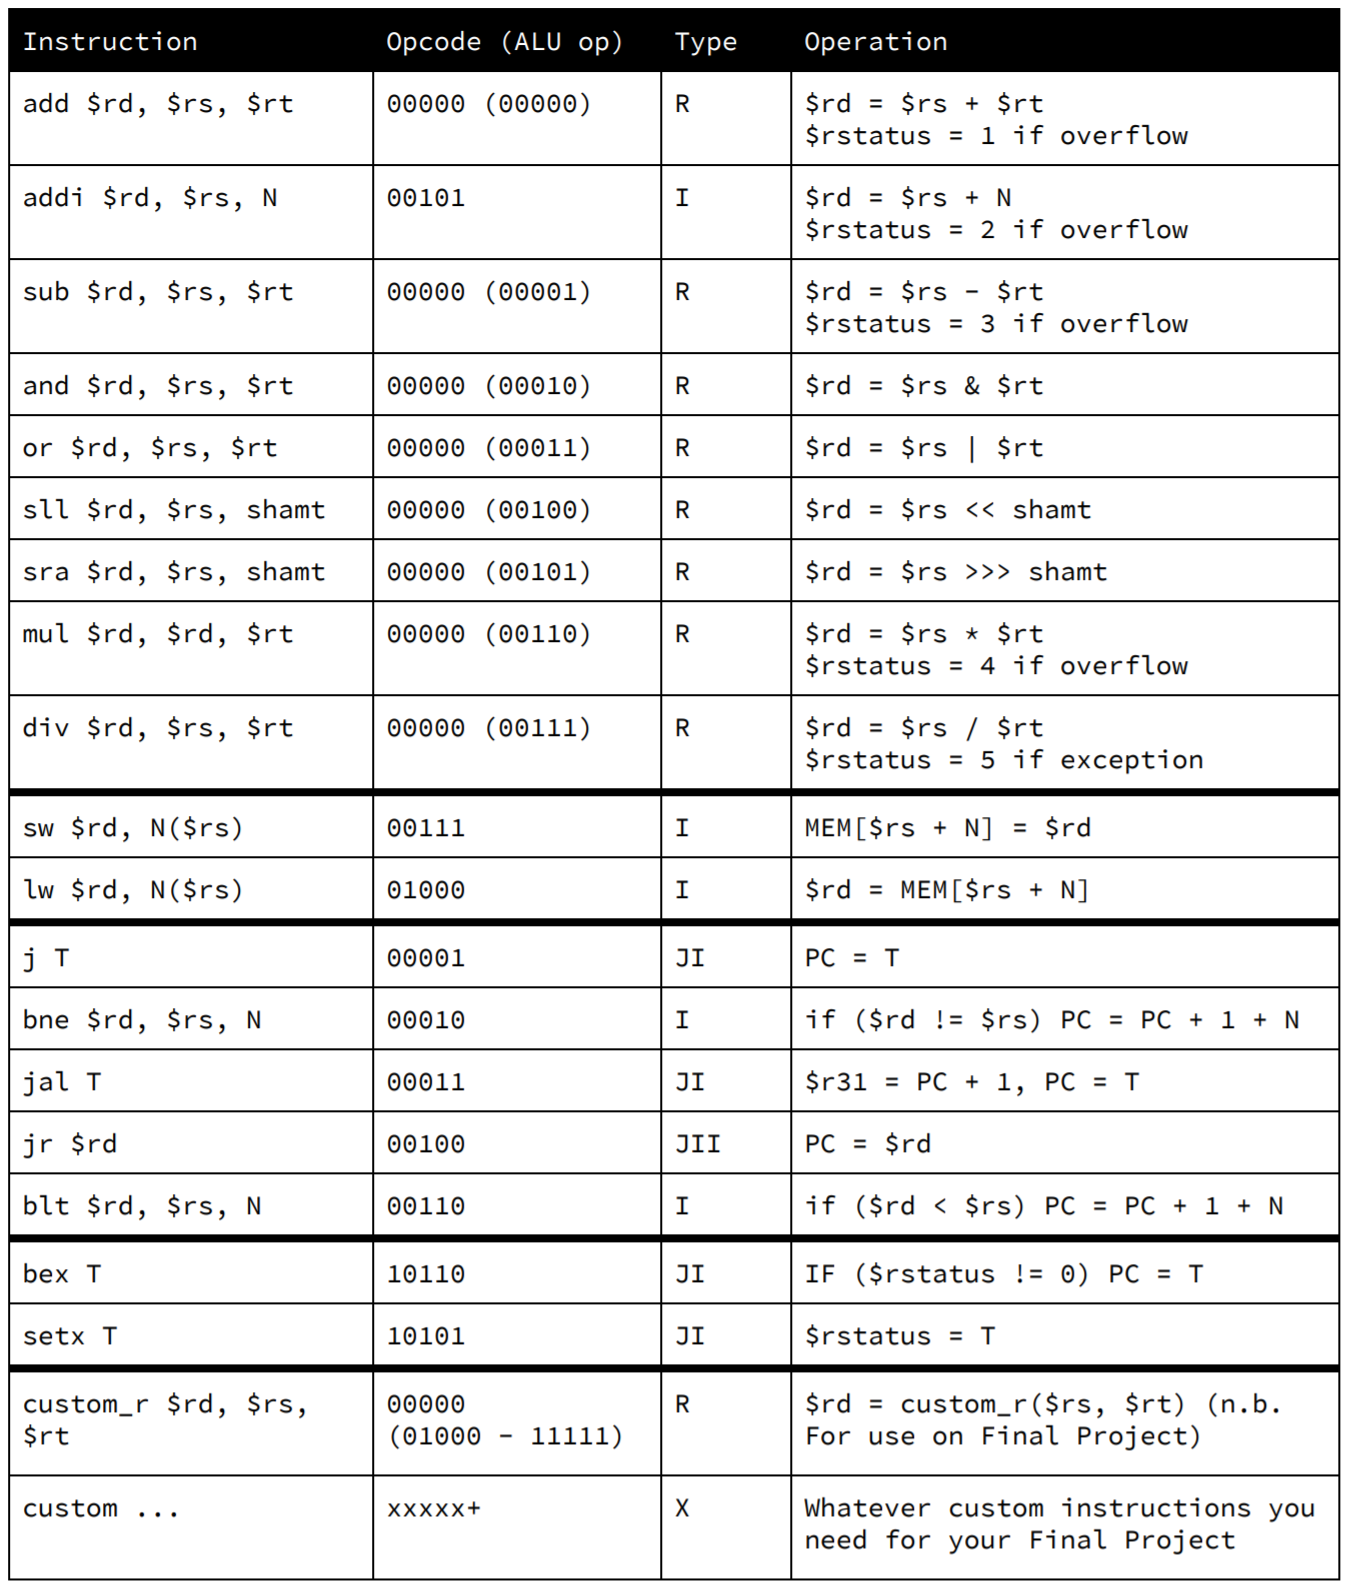
\includegraphics{ISA.PNG}
\caption{ECE 350 ISA}
\end{figure}

\begin{figure}[H]
\centering
\hspace*{-1cm} 
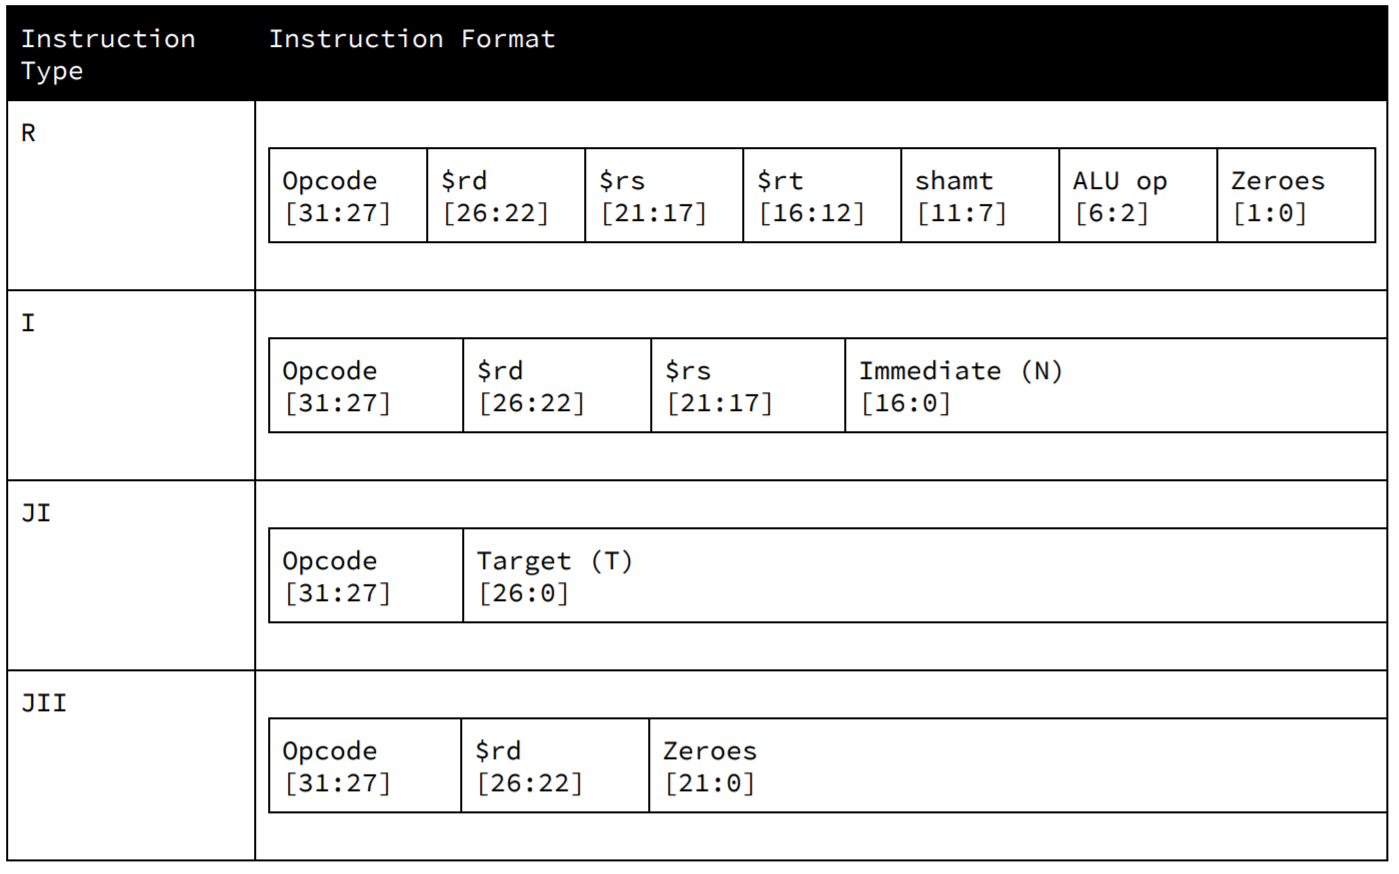
\includegraphics{TYPE.PNG}
\caption{Instruction Composition}
\end{figure}

\end{document}
